\section{Robot Implementation}
    
    \frame{\sectionpage}
    
    \begin{frame}{Robot program trigger phrases}
    	\begin{itemize}
    		\item "Give me a quote"
    		\item "I'd like a quote"
    		\item "Can I have a quote"
    	\end{itemize}
    \end{frame}
    
    \begin{frame}{Nao 6 Project Settings}
    	\begin{figure}
    		\centering
    		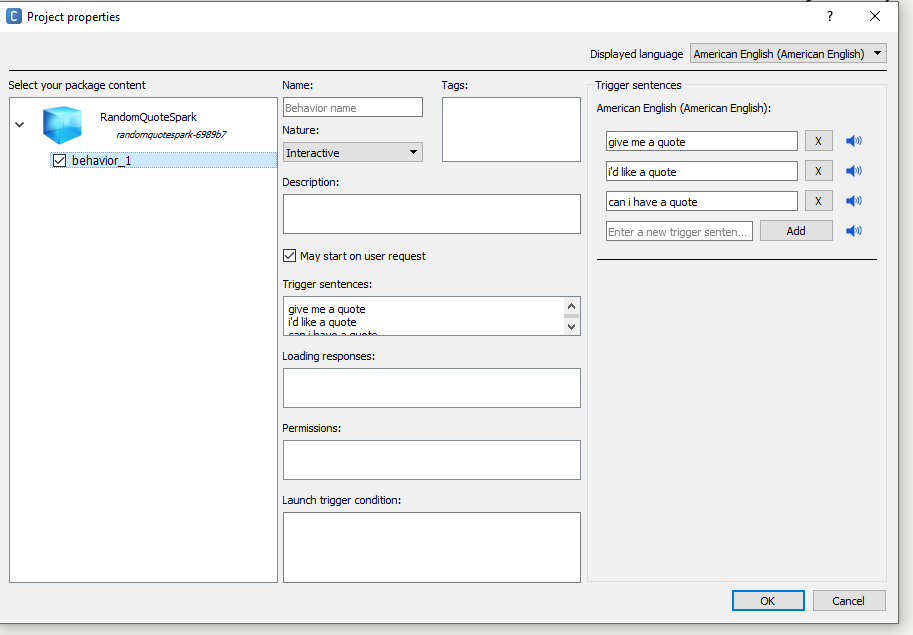
\includegraphics[width =0.7\linewidth]{robot-spark-proj/screenshot-3.PNG}
    		\caption{Robot trigger}
    	\end{figure}
    	
    \end{frame}
    
    \begin{frame}{Nao 6 Choreograph Program}
    	\begin{figure}
    		\centering
    		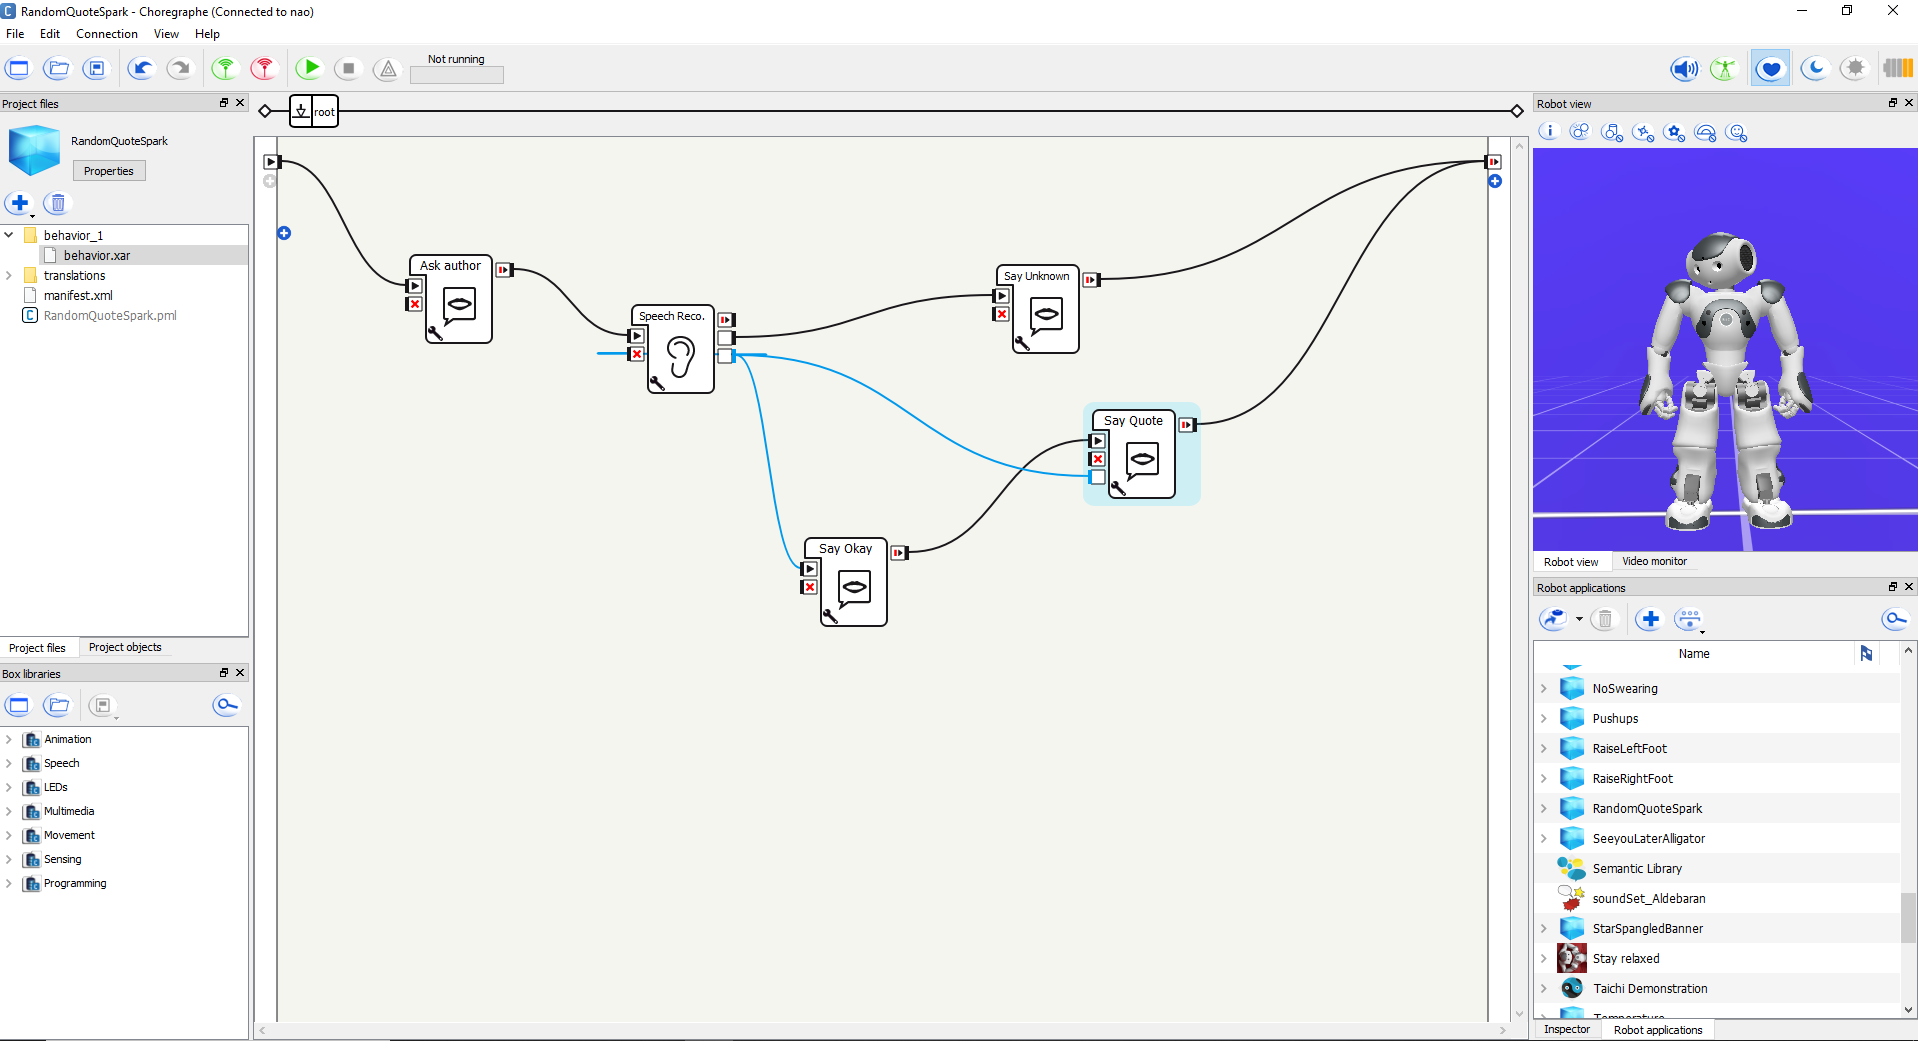
\includegraphics[width =1\linewidth]{robot-spark-proj/screenshot-1.PNG}
    		\caption{Diagram}
    	\end{figure}
    	
    \end{frame}


	\begin{frame}[fragile]{Robot Python2 - Server Request}
		\begin{verbatim}
		# Get request result from spark webserver
		r = requests.get("http://35.226.85.38:80/?author=" + 
		    str(author), timeout=5)
		
		# Convert request to json object
		data = r.json()
	
		# Say quote
		say = str(data['quote']) + ". " + str(data['author'])
		\end{verbatim}
	\end{frame}

\section{Live Demo}

\frame{\sectionpage}